\documentclass[a4paper]{article}

\usepackage{inputenc}
\usepackage[british,UKenglish]{babel}
\usepackage{amsmath}
%\usepackage{titlesec}
\usepackage{color}
\usepackage{graphicx}
\usepackage{fancyref}
\usepackage{hyperref}
\usepackage{float}
\usepackage{scrextend}
\usepackage{setspace}
\usepackage{xargs}
\usepackage{multicol}
\usepackage{nameref}

\usepackage{sectsty}
\usepackage{multicol}
\usepackage{multirow}
\usepackage[procnames]{listings}
\usepackage{appendix}

\newcommand\tab[1][1cm]{\hspace*{#1}}
\hypersetup{colorlinks=true, linkcolor=black}
\interfootnotelinepenalty=10000

\newcommand{\cleancode}[1]{\begin{addmargin}[3em]{3em}\texttt{\textcolor{cleanOrange}{#1}}\end{addmargin}}
\newcommand{\cleanstyle}[1]{\text{\textcolor{cleanOrange}{\texttt{#1}}}}


\usepackage[colorinlistoftodos,prependcaption,textsize=footnotesize]{todonotes}
\newcommandx{\commred}[2][1=]{\textcolor{Red}
{\todo[linecolor=red,backgroundcolor=red!25,bordercolor=red,#1]{#2}}}
\newcommandx{\commblue}[2][1=]{\textcolor{Blue}
{\todo[linecolor=blue,backgroundcolor=blue!25,bordercolor=blue,#1]{#2}}}
\newcommandx{\commgreen}[2][1=]{\textcolor{OliveGreen}{\todo[linecolor=OliveGreen,backgroundcolor=OliveGreen!25,bordercolor=OliveGreen,#1]{#2}}}
\newcommandx{\commpurp}[2][1=]{\textcolor{Plum}{\todo[linecolor=Plum,backgroundcolor=Plum!25,bordercolor=Plum,#1]{#2}}}

\def\code#1{{\tt #1}}

\def\note#1{\noindent{\bf [Note: #1]}}

\makeatletter
%% The "\@seccntformat" command is an auxiliary command
%% (see pp. 26f. of 'The LaTeX Companion,' 2nd. ed.)
\def\@seccntformat#1{\@ifundefined{#1@cntformat}%
   {\csname the#1\endcsname\quad}  % default
   {\csname #1@cntformat\endcsname}% enable individual control
}
\let\oldappendix\appendix %% save current definition of \appendix
\renewcommand\appendix{%
    \oldappendix
    \newcommand{\section@cntformat}{\appendixname~\thesection\quad}
}
\makeatother


% "define" Scala
\usepackage[T1]{fontenc}  
\usepackage[scaled=0.82]{beramono}  
\usepackage{microtype} 

\sbox0{\small\ttfamily A}
\edef\mybasewidth{\the\wd0 }

\lstdefinelanguage{scala}{
  morekeywords={abstract,case,catch,class,def,%
    do,else,extends,false,final,finally,%
    for,if,implicit,import,match,mixin,%
    new,null,object,override,package,%
    private,protected,requires,return,sealed,%
    super,this,throw,trait,true,try,%
    type,val,var,while,with,yield},
  sensitive=true,
  morecomment=[l]{//},
  morecomment=[n]{/*}{*/},
  morestring=[b]",
  morestring=[b]',
  morestring=[b]"""
}

\usepackage{color}
\definecolor{dkgreen}{rgb}{0,0.6,0}
\definecolor{gray}{rgb}{0.5,0.5,0.5}
\definecolor{mauve}{rgb}{0.58,0,0.82}

% Default settings for code listings
\lstset{frame=tb,
  language=scala,
  aboveskip=3mm,
  belowskip=3mm,
  showstringspaces=false,
  columns=fixed, % basewidth=\mybasewidth,
  basicstyle={\small\ttfamily},
  numbers=none,
  numberstyle=\footnotesize\color{gray},
  % identifierstyle=\color{red},
  keywordstyle=\color{blue},
  commentstyle=\color{dkgreen},
  stringstyle=\color{mauve},
  frame=single,
  breaklines=true,
  breakatwhitespace=true,
  procnamekeys={def, val, var, class, trait, object, extends},
  procnamestyle=\ttfamily\color{red},
  tabsize=2
}

\lstnewenvironment{scala}[1][]
{\lstset{language=scala,#1}}
{}
\lstnewenvironment{cpp}[1][]
{\lstset{language=C++,#1}}
{}
\lstnewenvironment{bash}[1][]
{\lstset{language=bash,#1}}
{}
\lstnewenvironment{verilog}[1][]
{\lstset{language=verilog,#1}}
{}



\lstset{frame=,basicstyle={\footnotesize\ttfamily}}



\graphicspath{ {images/} }
\usepackage{ctex}
\usepackage{verbatim}
\usepackage{geometry}
\usepackage{amsmath}
\usepackage{pifont}%\ding{192} \ding{172}
\usepackage{tikz}
\usepackage{float}
\usepackage{booktabs}
\usepackage{bm}
%\geometry{a4paper, scale=0.72}
\geometry{a4paper,left=2.5cm,right=2.5cm,top=2.5cm,bottom=2.5cm}
%%%%%%%%%%%%%%%%%%%%%%%%%%%%%%%%%%%%%%%% BEGIN DOC %%%%%%%%%%%%%%%%%%%%%%%%%%%%%%%%%%%%%%%%

\begin{document}
\renewcommand{\contentsname}{目\ 录}
\renewcommand{\appendixname}{附录}
\renewcommand{\appendixpagename}{附录}
\renewcommand{\refname}{参考文献} 
\renewcommand{\figurename}{图}
\renewcommand{\tablename}{表}
\renewcommand{\today}{\number\year 年 \number\month 月 \number\day 日}
\newcommand{\refeq}[1]{\textbf{Eq.(\ref{#1})}}
\newcommand*{\circled}[1]{\lower.7ex\hbox{\tikz\draw (0pt, 0pt)%
    circle (.5em) node {\makebox[1em][c]{\small #1}};}}
    
\title{{\Huge 近代物理实验报告{\large\linebreak\\}}{\Large 实验2-6:\ 用$\beta$粒子检验相对论的动量-动能关系\linebreak\linebreak}}
%please write your name, Student #, and Class # in Authors, student ID, and class # respectively
\author{\\姓\ 名:付\ 大\ 为\\
学\ 号: 1800011105\\
邮\ 箱: \url{fudw@pku.edu.cn}\\
%班\ 号: xxxxx\\\\
近代物理实验 (I)\\
(2021,秋季学期)\\\\
北京大学\\
物理学院\\
2018级1班}
\date{\today}
\maketitle
\newpage

%%%%%%%%%%%%%%%%%%%%%%%%%%%%%%%%%%%%%%%% ABSTRACT %%%%%%%%%%%%%%%%%%%%%%%%%%%%%%%%%%%%%%%%
\begin{center}
{\Large\bf{摘\ 要\\}}
\end{center}

经典力学和电磁学以及光学之间的矛盾,促成了狭义相对论理论的诞生.狭义相对论理论对于高速物体的运动,和经典力学对于物体的动量-动能关系,给出了不同的预言.本实验通过测量高能$\beta$粒子的动量和动能,验证了狭义相对论对于高速运动物体动量-动能关系的预言.本实验旨在从动量--能量关系这一角度,验证这相对论的准确性.实验中使用$\beta$源产生速度接近光速的$\beta$粒子,通过分别测定其动量、能量,分析其动量--能量关系,验证了狭义相对论的预测.
\\\\
{\bf{关键词}:}\ 狭义相对论,动量-动能关系,$\ \beta$衰变,$\ \beta$粒子
\newpage

%%%%%%%%%%%%%%%%%%%%%%%%%%%%%%%%%%%%%%%% CONTENT %%%%%%%%%%%%%%%%%%%%%%%%%%%%%%%%%%%%%%%%
\begin{center}
\tableofcontents\label{c}
\end{center}
\newpage

%%%%%%%%%%%%%%%%%%%%%%%%%%%%%%%%%%%%%%%% Introduction %%%%%%%%%%%%%%%%%%%%%%%%%%%%%%%%%%%%%%%%
\section{引言} \label{overview}%------------------------------
经典力学对于低速物体的运动规律进行了彻底的研究并且获得了相当的成功,它反
映了牛顿的绝对时空观.绝对时空观认为时间和空间彼此独立,没有联系.时间与空
间的度量与惯性参考系的运动状态无关.同时,认为同一物体在不同惯性参考系中
的运动量按照一定的变换规律互相联系(伽利略变换),并且一切力学定律的表达式
在一切惯性系中都是一样的(力学相对性原理).

直到19世纪末到20世纪初,人们试图将伽利略变换和力学相对性原理推广到电磁学
与光学,但遇到了巨大的困难与矛盾.实验表明,对于高速运动的物体,伽利略变换
是不正确的,并且实验还证明,在所有惯性参考系中,光在真空中的传播速度均为同
一常数.在这些实验基础上,爱因斯坦在1905年基于两条原理,即爱因斯坦相对性原
理和光速不变原理,建立了狭义相对论,将仅仅局限于力学的伽利略相对性原理推
广到包括电磁学和光学的整个物理学.

$\beta$射线在穿过物质时可以通过以下过程损失能量:在介质内不断产生电子-离子对的电离作用导致其部分或全部动能消耗,即使穿过的介质非常薄,通常也有能量衰减; $\beta$射线可能被原子核和电子的库仑势散射,在损失能量的同时还将影响自身的运动方向;当$\beta$射线受介质库仑场作用做减速运动时,一部分动能会通过韧致辐射以光子的形式发射;如果$\beta$射线本身的运动速度超过光在当前介质中的传播速度,则可通过切伦科夫光的形式损失动能.

动能测定通过 NaI (Tl) \textbf{闪烁体探测器}实现。入射粒子的动能传递给闪烁体使之激发、退激,放出光子(\textit{闪烁}),经光电倍增、前置放大、线性放大等步骤,转化为充分强的电脉冲输入\textbf{多道分析器};多道分析器将脉冲强度转化为道址$n$存储并计数。

本次实验中,光电倍增管加高压$U = \SI{585}{\V}$. 注意,上述能量转换过程基本上是线性的,即有$n\propto E$;利用标准放射源$\mathrm \sideset{^{60}}{}Co$和$\mathrm \sideset{^{137}}{}Cs$ 进行定标,可进一步确定$n$--$E$关系,由此获得粒子的动能.

在出射窗与探测器之间,放入不同厚度的铝膜对狭缝进行遮挡,测量铝膜衰减后的$\beta$多道能谱,研究铝膜对能谱形状的影响.利 用$\mathrm \sideset{^{60}}{}Co$及$\mathrm \sideset{^{137}}{}Cs$的$\gamma$特征射线对系统进行能量刻度.拟合各$\beta$多道能谱的信号峰给出峰位,从而计算动量和动能大小.

狭义相对论对于速度接近光速$c$的高速运动物体的运动学和动力学,给出了与经
典力学完全不同的预计.本实验旨在通过测量高能量$\beta$粒子的动量-能量关
系,来验证狭义相对论理论对于这一关系的预计,从而验证狭义相对论这一理论自
身的正确性.

%%%%%%%%%%%%%%%%%%%%%%%%%%%%%%%%%%%%%%%% Theory %%%%%%%%%%%%%%%%%%%%%%%%%%%%%%%%%%%%%%%%
\newpage
\section{理论} \label{theory}%------------------------------
狭义相对论的理论框架基于如下两个假设建立:

\begin{enumerate}
\item 爱因斯坦相对性原理: 所有物理规律在所有惯性参考系中具有完全相同的
  形式.
\item 光速不变原理: 在所有惯性参考系中光在真空的速度恒定为$c$,它与光源
  和参考系的运动无关.
\end{enumerate}

基于这两个假设,可以推导出洛伦兹变换.洛伦兹变换作为一种变换关系,用于联系不同惯性参考系之中的运动量.同时,如若引入$x_1 = x, x_2 = y, x_3 = z,x_4 = ict$,根据洛伦兹变换,可以发现在变换中存在一个不变量$x_1^2 + x_2^2+ x_3^2 + x_4^2$,从而洛伦兹变换可以看成复四维时空$(x_1, x_2, x_3,x_4)$之中的转动.

另一方面,根据相对性原理,任何物理规律在不同的惯性系中都具有相同的形式,因此表达物理规律的方程必须满足在洛伦兹变换形式下不变,称为洛伦兹变换的协变性.由于洛伦兹变换可以看成上述复四维时空中的转动,因此,若能将物理量和物理规律的表达式以该四维时空中的形式进行表述,可以使得表述本身更加清晰、简明.

首先,四维时空中的坐标平方和以及微位移平方都是洛伦兹不变量,即
\begin{equation}
  \label{eq:const1}
  x_1^2 + x_2^2 + x_3^2 + x_4^2 = \text{const.}
\end{equation}

以及
\begin{equation}
  \label{eq:const2}
  (dx_1)^2 + (dx_1)^2 + (dx_1)^2 + (dx_1)^2 = \text{const.}
\end{equation}

从这个角度上来看,由于洛伦兹变换是四维时空中的转动,因此可以定义四维位矢和四维微位移,即
\begin{equation}
  \label{eq:4vecr}
  \bm{R} = (x,y,z,ict)
\end{equation}

以及
\begin{equation}
  \label{eq:4vecdr}
  d\bm{R} = (dx,dy,dz,icdt)
\end{equation}

那么,作为这些矢量的长度平方,前述的两个量自然在洛伦兹变换下不变.

进一步根据狭义相对论的动力学,可以得出四维时空形式下的动量矢量的表达式应为
\begin{equation}
  \label{eq:4vecp}
  \bm{P} = (P_1, P_2, P_3, P_4) =  (mv_1,mv_2,mv_3, \frac{i}{c}E)
\end{equation}

其中,$m = \frac{m_0}{\sqrt{1-v^2/c^2}}$为物体质量,$v_1,v_2,v_3$为物体速度在空间$x,y,z$三个轴向的分量,$E=mc^2$为物体的总能量.


取一个运动物体的随体系和实验室系之间的洛伦兹变换,由式~\ref{eq:4vecp}描述的变换不变性,可以得到
\begin{equation}
  \label{eq:E-P}
  E^2 - c^2p^2 = E_0^2
\end{equation}

即得到动能-动量关系
\begin{equation}
  \label{eq:Ek-P}
  E_k = E - E_0 = \sqrt{c^2p^2 + m_0^2c^4} - m_0c^2
\end{equation}

可以注意到,当$\frac{v}{c} \ll 1$时,动量-能量关系退化到经典形式,即
\begin{equation}
  \label{eq:classical}
  E_k = mc^2 - m_0c^2 = m_0c^2(\frac{1}{\sqrt{1-v^2/c^2}} - 1) =
  m_0c^2(1 + \frac{1}{2}\frac{v^2}{c^2} + \cdots) - m_oc^2 \simeq
  \frac{1}{2}m_0v^2 = \frac{p^2}{2m_0}
\end{equation}
%%%%%%%%%%%%%%%%%%%%%%%%%%%%%%%%%%%%%%%% Experiment %%%%%%%%%%%%%%%%%%%%%%%%%%%%%%%%%%%%%%%%
\newpage
\section{实验} \label{experiment}%------------------------------

\subsection{实验仪器}\label{sub:sysover}
\begin{itemize}
\item{\textbf{Sr-Y$\ \beta$源}}
\item{\textbf{真空泵}}
\item{\textbf{多道分析器}}
\item{\textbf{闪烁探头}}
\item{\textbf{高压电源}}
\item{\textbf{真空盒}}
\item{\textbf{磁谱仪(如下图\ref{fig:fig1})}}
\begin{figure}[ht]
 \centering
 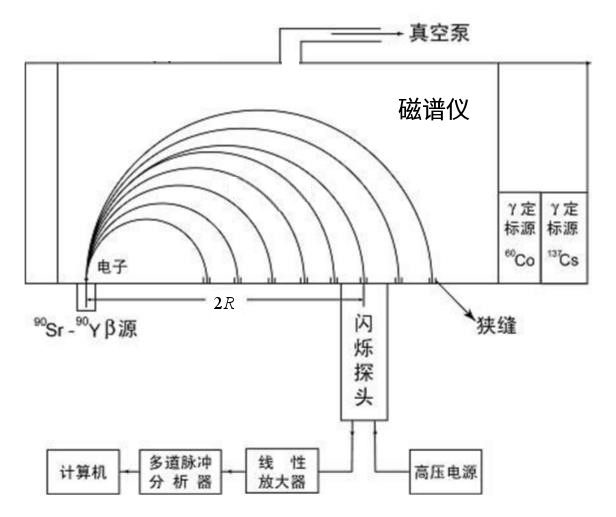
\includegraphics[height=12cm, width=14cm]{images/app.png}
 \caption{实验装置图}
 \label{fig:fig1}
\end{figure}\\\\
\end{itemize}

\newpage
\subsection{简要实验步骤}\label{sub:ExperimentalSteps}
分为以下几个步骤:\\\\
\circled{1}抽真空(按橘色按钮),约2分钟,机械泵声音平稳即可\\\\
\circled{2}将探测器的狭缝放最后一个窗,调节探测的高压(小于600V)或放大倍数,使得$\beta$的信号峰在屏幕的最右端完整显示出来\\\\
\circled{3}在真空状态下,将探测器放2$\sim$8号窗,分别测量能谱,记下活时间及能谱(最后转为文本文件以便分析),以便计算信号的计数率.等待的过程中进行蒙特卡洛模拟.\\\\
\circled{4}关掉真空泵按钮。在等待真空盒进入空气的过程中,利用$\gamma$源进行探测器刻度。\\\\
\circled{5}等真空表指示为0的时候,在真空盒充满空气状态下重复步骤3。等待的过程中进行蒙特卡洛模拟。比较同一位置空气及真空下的计数率,测量各窗能谱\\\\
\circled{6}进行能谱分析给出峰位,给出动量及动能关系图,写实验报告\\\\



%%%%%%%%%%%%%%%%%%%%%%%%%%%%%%%%%%%%%%%% Results & Discussions %%%%%%%%%%%%%%%%%%%%%%%%%%%%%%%%%%%%%%%%
\newpage
\section{结果及讨论}
%------------------------------------------------------------
\subsection{用$\sideset{^{60}}{}{\mathrm{Co}}$和$\sideset{^{137}}{}{\mathrm{Cs}}$对探测器进行能量刻度}\label{sub:1}
在活时间$T=300s$的设置下,测出$\sideset{^{60}}{}{\mathrm{Co}}$与$\mathrm \sideset{^{137}}{}Cs$放射源的能谱图,并找到对应的光电峰,如下图\ref{fig:fig2}. 
\begin{figure}[H]
 \centering
 \caption{$\mathrm \sideset{^{60}}{}{Co}$与$\mathrm \sideset{^{137}}{}{Cs}$的光电峰}
 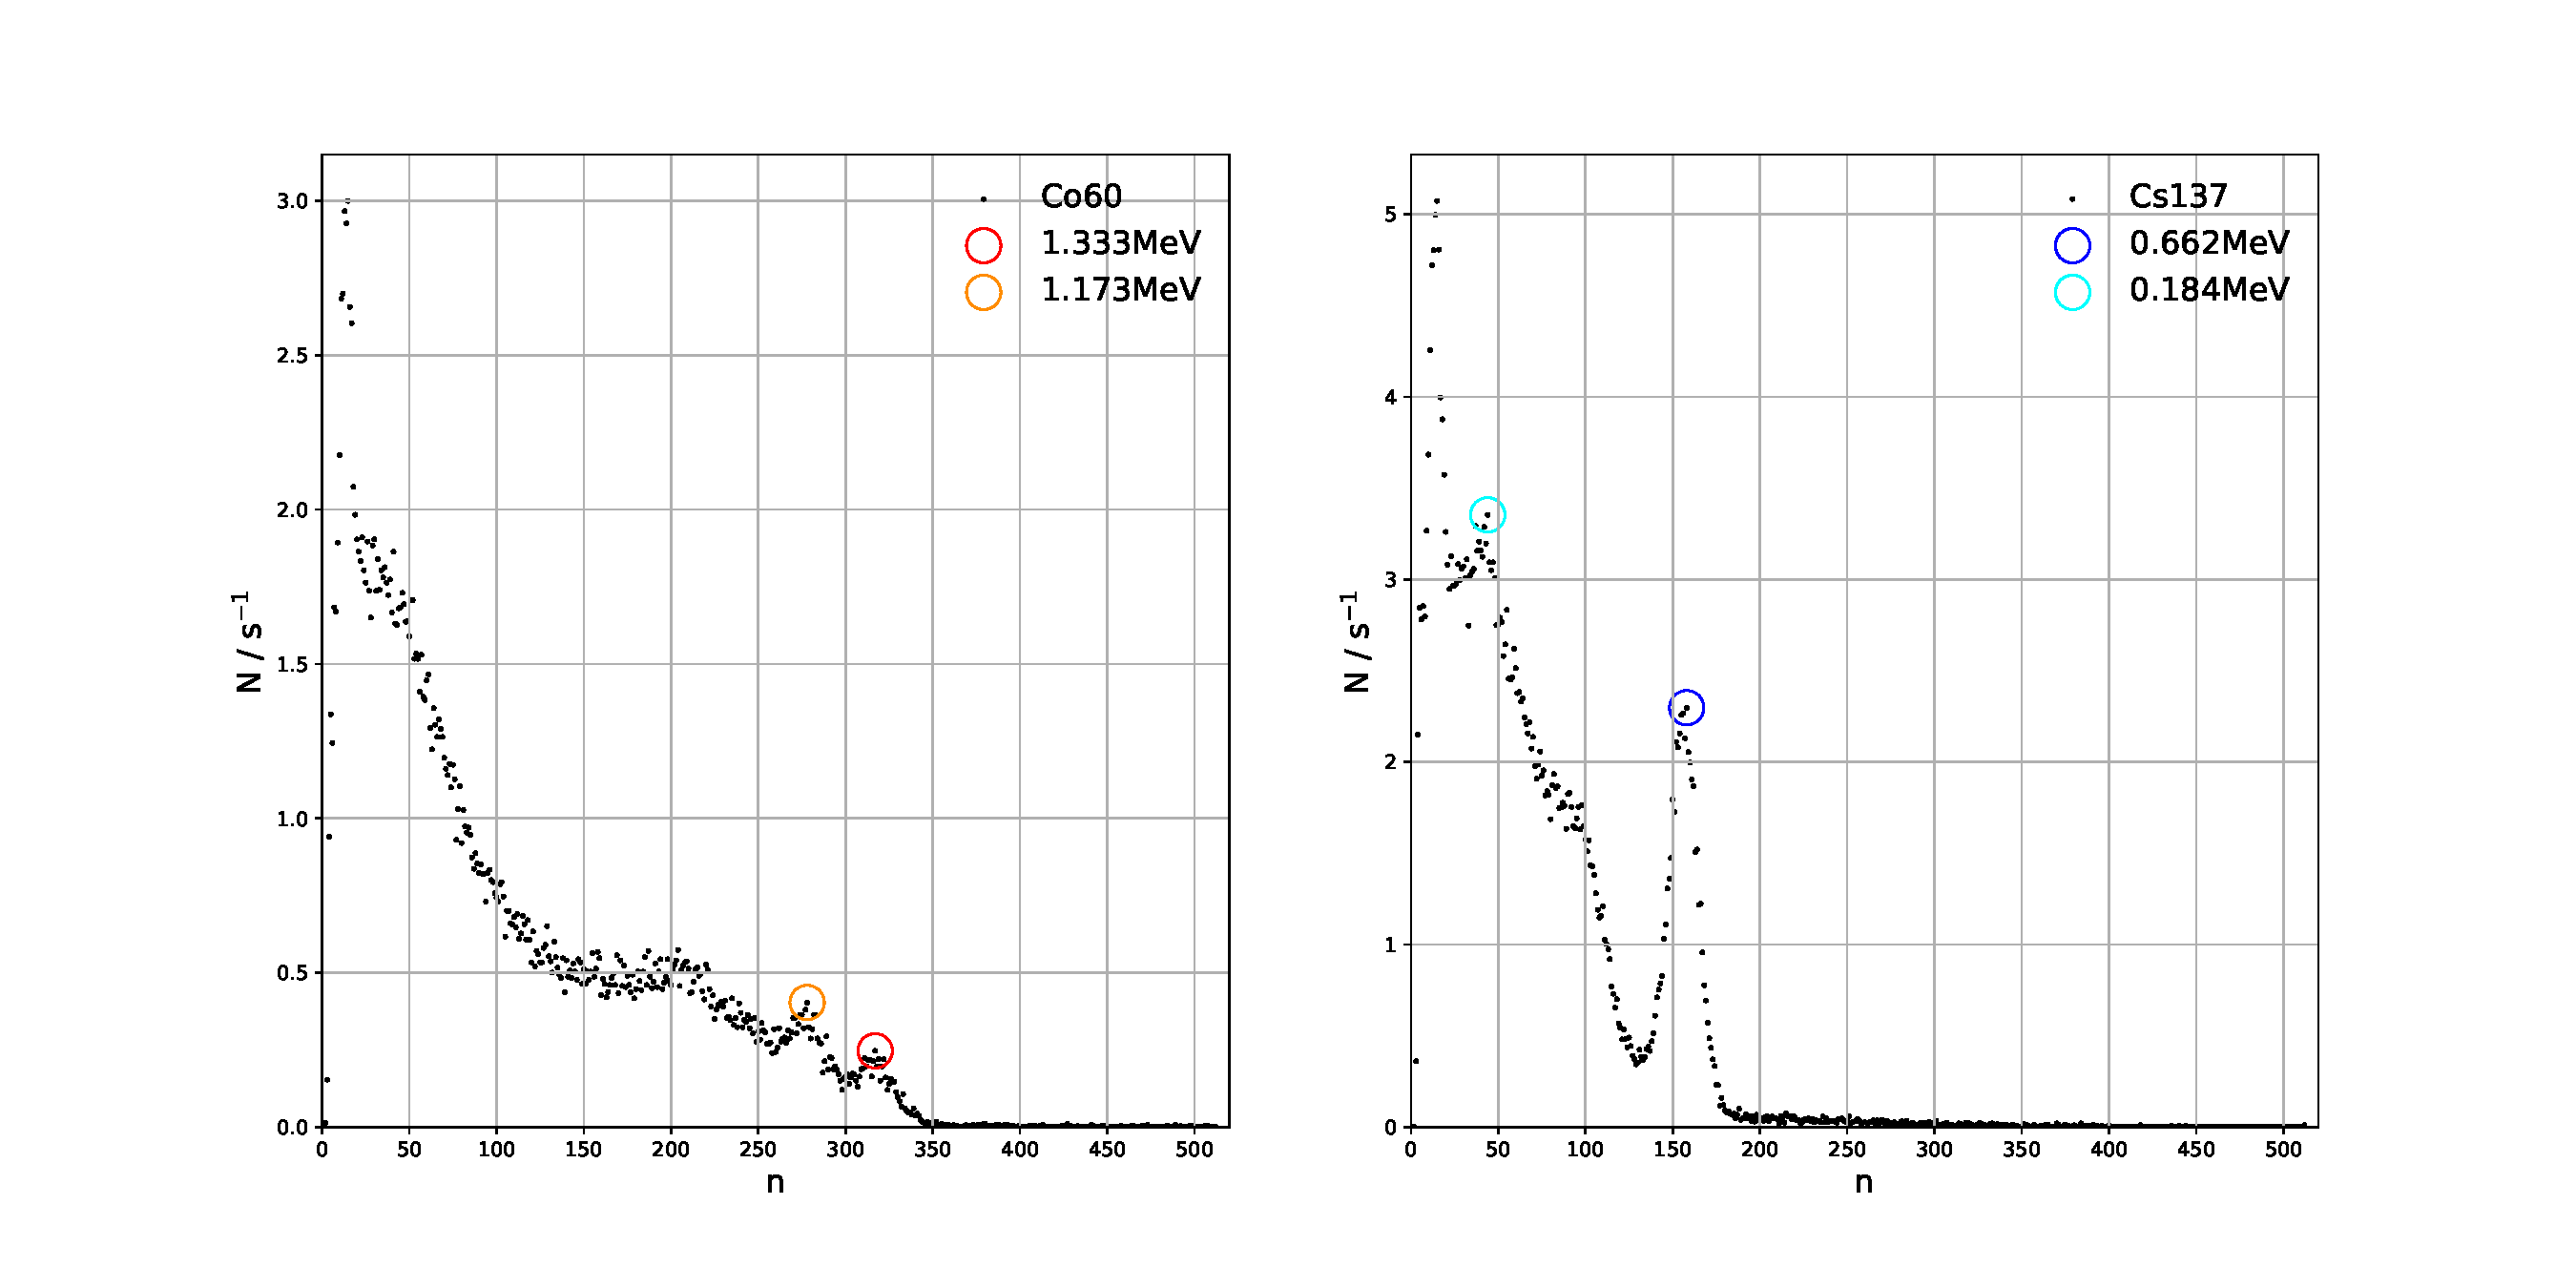
\includegraphics[height=8cm, width=16cm]{images/phyex3_fig1.pdf}
 \label{fig:fig2}
\end{figure}
可以得到入射光子的动能$E_k$与道数n的对应关系如下\textbf{表\ref{tab:1}}
\begin{table}[htp]
\caption{道数n与动能$E_k$定量关系}\label{tab:1}
\setlength{\tabcolsep}{7mm}
\begin{center}\begin{tabular}{|c|c|}
	\toprule \hline
	\textbf{道数$\rm n$} & \textbf{入射光子子动能$\rm E_k/MeV$}\\ \hline \hline
	$44$    & $0.184$ 	\\ \hline
	$158$    & $0.662$    \\ \hline
	$278$    & $1.173$    \\ \hline
	$317$    & $1.333$    \\ \hline
	\bottomrule
	\end{tabular}
\end{center}
\end{table}

然后通过最小二乘法直线拟合得到探测器刻度关系,拟合后得到的能量与道数直线关系为
\begin{equation}\label{eq:E-x}
    E=[(0.0422\pm0.00001)n+(-0.00234\pm0.00294)]\rm MeV
\end{equation}

如下\textbf{图\ref{fig:fig3}}所示.
\begin{figure}[H]
 \centering
 \caption{利用$\mathrm \sideset{^{60}}{}Co$源和$\mathrm \sideset{^{137}}{}Cs$源对探测器刻度}
 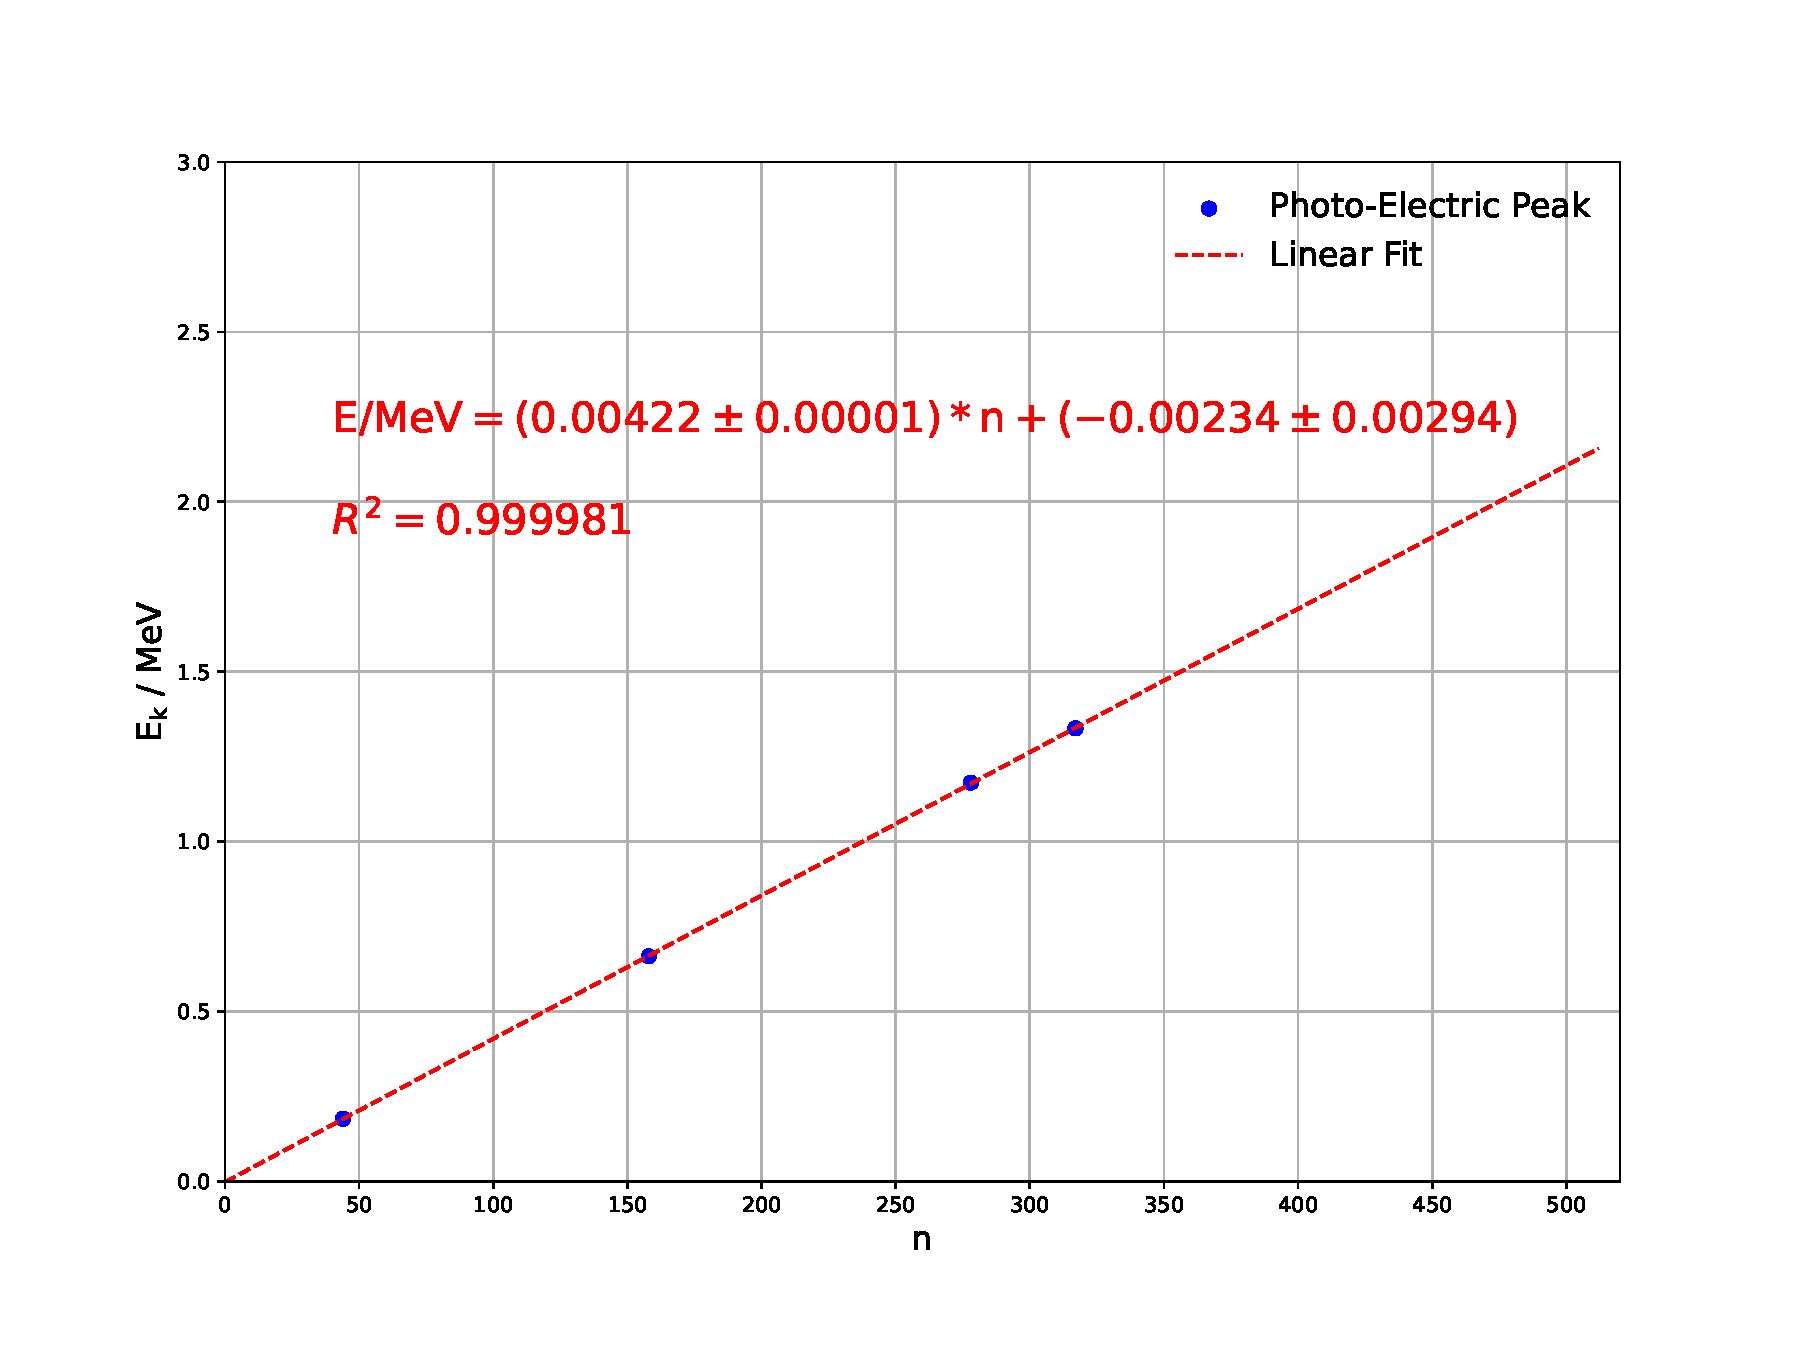
\includegraphics[height=12cm, width=16cm]{images/phyex3_fig2.pdf}
 \label{fig:fig3}
\end{figure}
上图可以看出定标结果说明能量和道数的线性关系符合得非常好.
\begin{comment}
如果需要索引参考文献,请使用\cite{Erdos01}, 同时已经将参考文献的项目模版在文末写出。
\end{comment}
%------------------------------------------------------------
\newpage
\subsection{在真空状态下,测量出峰位处$\beta$粒子的动量和动能大小}\label{sub:2}
\subsubsection{测出2$\sim$8窗的$\beta$能谱和峰位置}\label{sub:2-1}
首先在活时$T=300s$的设置下,测出如真空状态各窗的能谱分布,并且用高斯函数拟合峰部以得到峰位置,如下\textbf{图\ref{fig:fig4}}所示. 
\begin{figure}[H]
 \centering
 \caption{真空状态下2$\sim$8窗的能谱图和高斯拟合峰}
 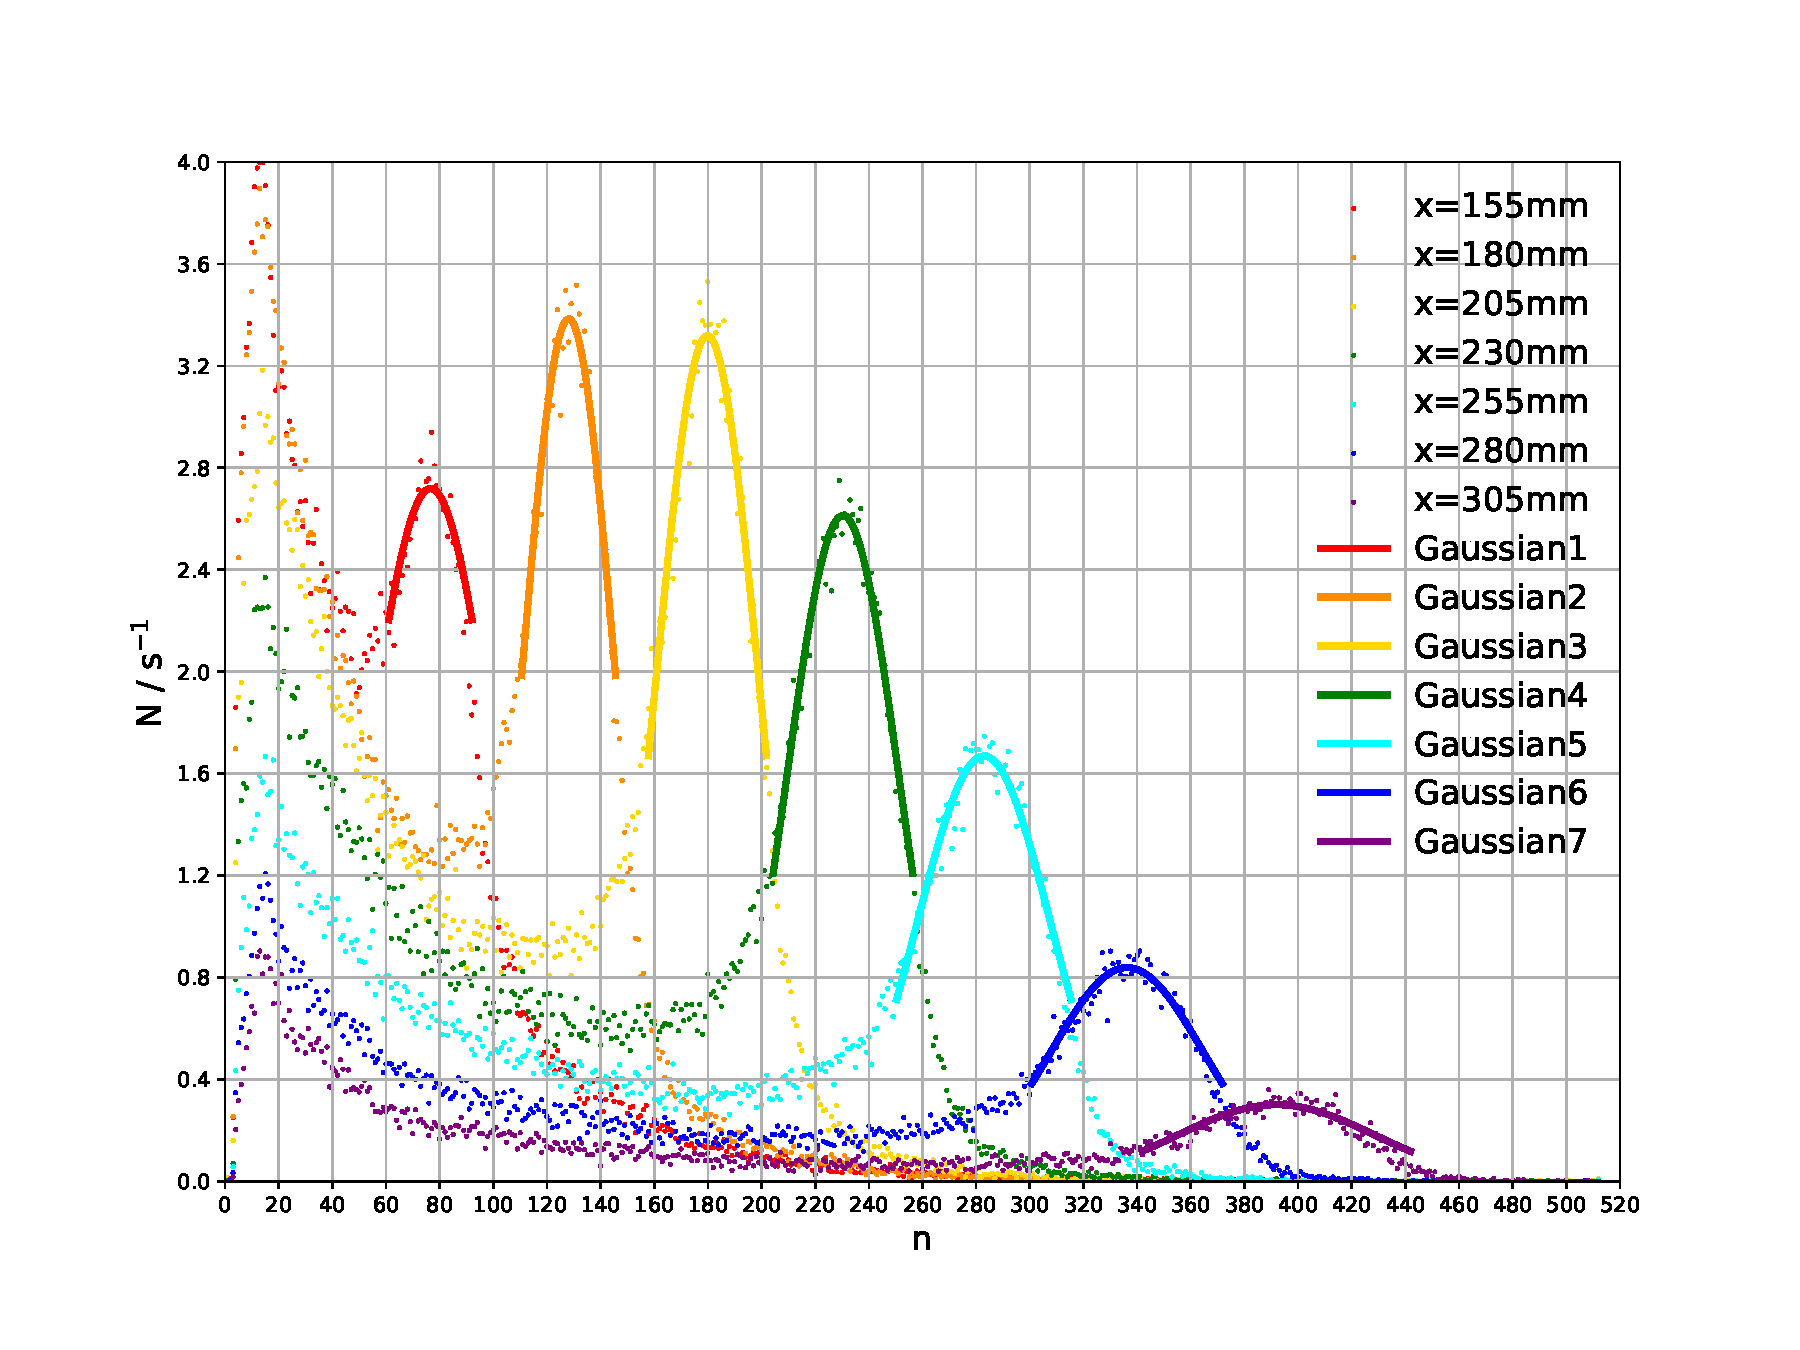
\includegraphics[height=12cm, width=16cm]{images/phyex1_fig1.pdf}
 \label{fig:fig4}
\end{figure}
\subsubsection{通过峰位置计算动量和动能大小}\label{sub:2-2}
通过探测器构造,$\beta$源位置为$x_0=60mm$,则我们知道打到窗口距离$x$处的粒子的磁场回旋半径$R=(x-x_0)/2$,这样可以通过粒子在磁场中的回旋计算得到其动量大小为
\begin{equation}
    \left|\vec {p}\right|=q_{\beta}BR=\frac{eB(x-x_0)}{2}
\end{equation}

更进一步,通过\textbf{~\ref{sub:1}节}中的能量定标公式\refeq{eq:E-x},我们可以计算得到探测到的能量如下
\begin{equation*}
    E=[(0.0422\pm0.00001)n+(-0.00234\pm0.00294)]\rm MeV \eqno{(7)}
\end{equation*}

考虑Al膜和有机膜的能量损失修正,根据线性内插进行计算得到$\beta$粒子动能$E_k$

综上我们可以得到不同窗口处接收到的$\beta$粒子的动量能量关系如下\textbf{表\ref{tab:2}}
\begin{table}[H]
\setlength{\tabcolsep}{3mm}
\caption{真空状态不同窗$\beta$粒子动量大小$pc$和动能$E_k$关系}\label{tab:2}
\begin{center}\begin{tabular}{|c|c|c|c|c|}
	\toprule
	\hline
	\textbf{窗号} & \textbf{峰位置道数$n$} & \textbf{探测到的能量$E/\rm MeV$} & \textbf{$\beta$粒子动能$E_k/\rm MeV$} & \textbf{$\beta$粒子动量$pc/\rm MeV$}\\ \hline \hline
	$2$ & $76.58$ & 0.321 & 0.439 & 0.846\\ \hline
	$3$ & $128.09$ & 0.538 & 0.638 & 1.072\\ \hline
	$4$ & $179.83$ & 0.756 & 0.853 & 1.298\\ \hline
	$5$ & $230.33$ & 0.969 & 1.065 & 1.524\\ \hline
	$6$ & $282.88$ & 1.190 & 1.284 & 1.750\\ \hline
	$7$ & $336.25$ & 1.416 & 1.510 & 1.976\\ \hline
	$8$ & $391.88$ & 1.650 & 1.745 & 2.202\\ \hline
	\bottomrule
	\end{tabular}
\end{center}
\end{table}
%------------------------------------------------------------
\newpage
\subsection{在空气状态下,测量出峰位处$\beta$粒子的动量和动能大小}\label{sub:3}
\subsubsection{测出2$\sim$8窗的$\beta$能谱和峰位置}\label{sub:3-1}
首先在活时$T=300s$的设置下,测出如真空状态各窗的能谱分布,并且用高斯函数拟合峰部以得到峰位置,如下\textbf{图\ref{fig:fig5}}所示. 
\begin{figure}[H]
 \centering
 \caption{空气状态下2$\sim$8窗的能谱图和高斯拟合峰}
 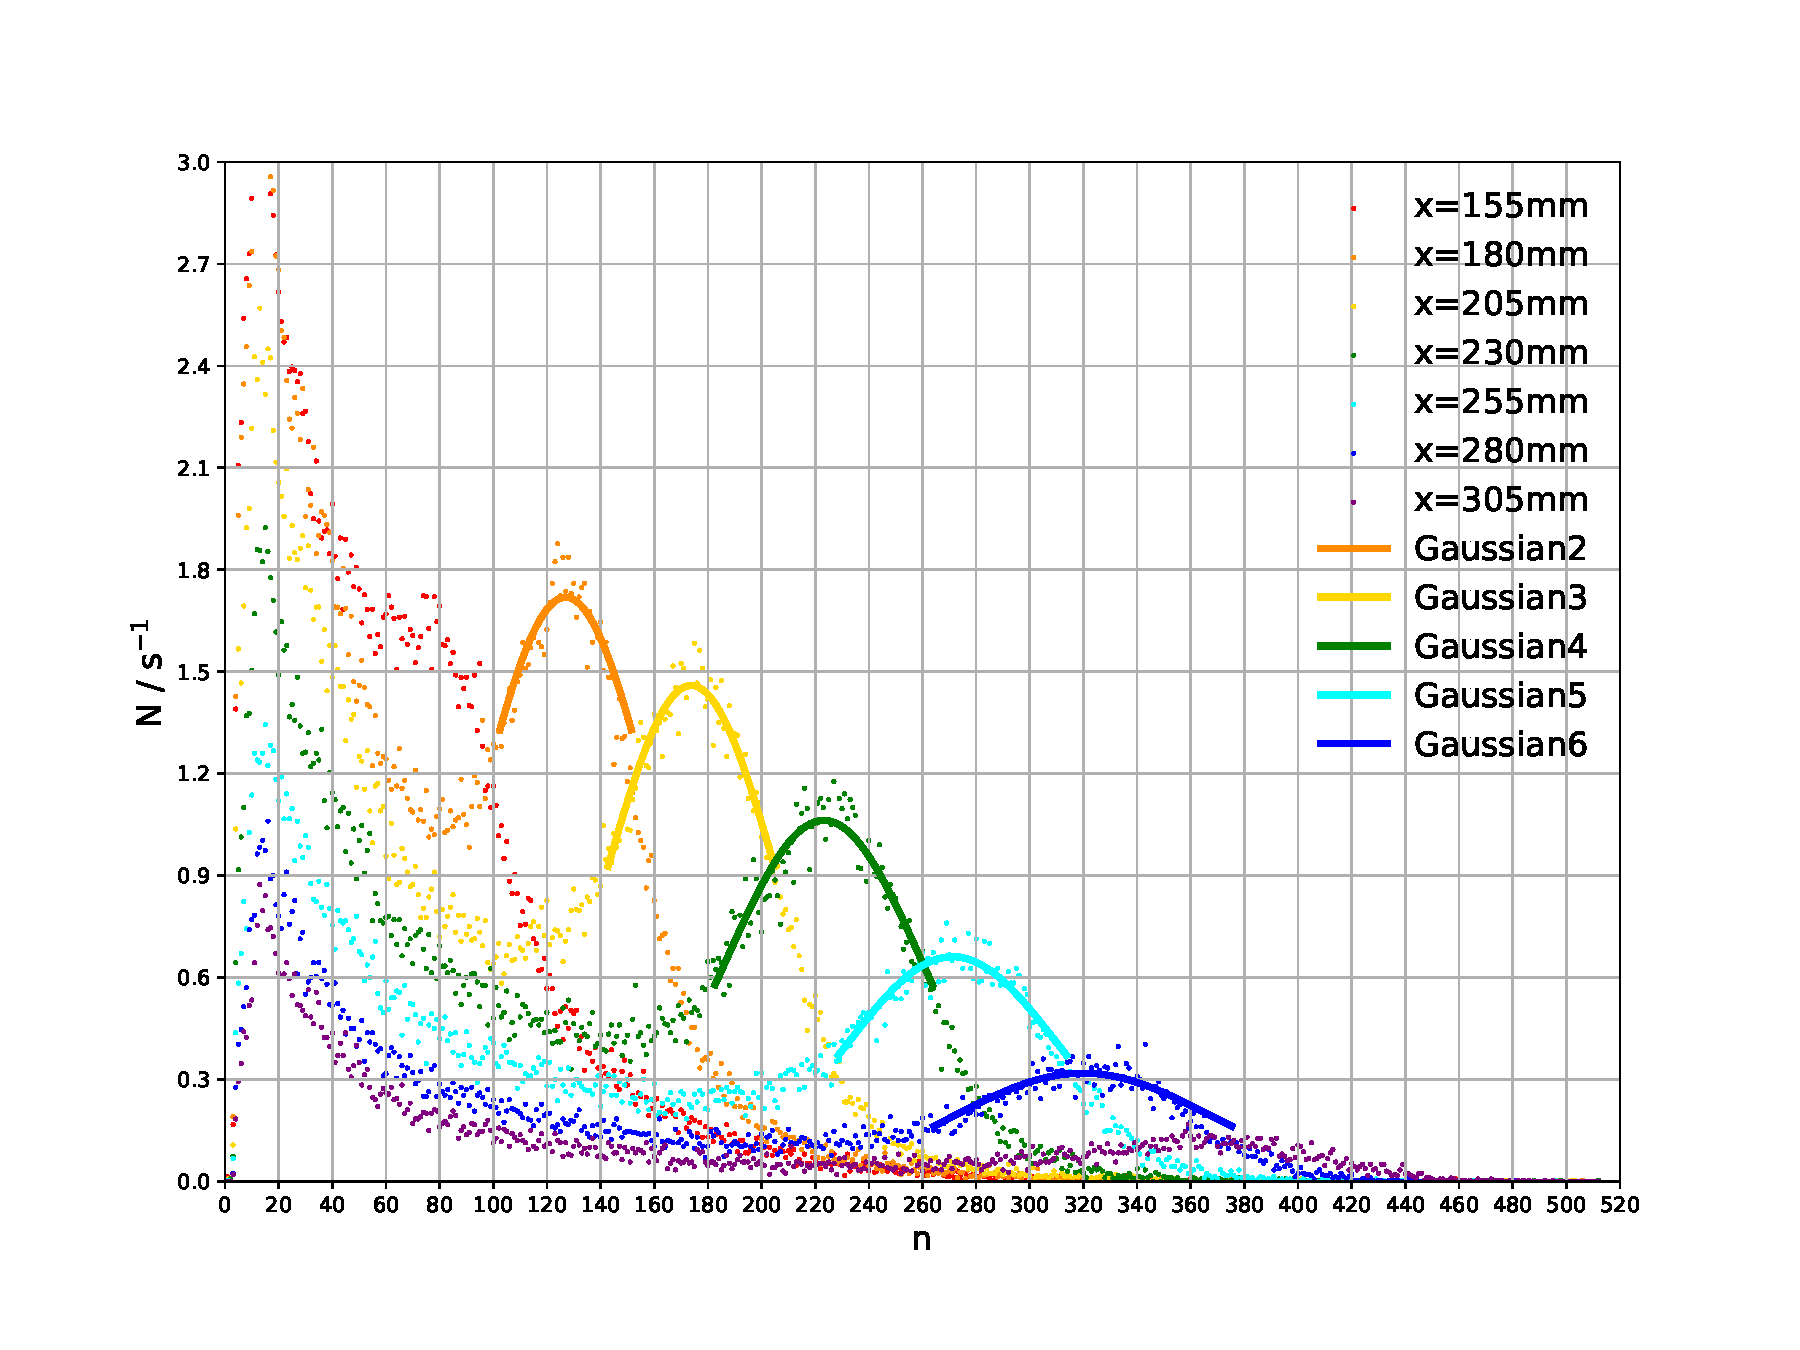
\includegraphics[height=12cm, width=16cm]{images/phyex2_fig1.pdf}
 \label{fig:fig5}
\end{figure}
值得注意的是,这里我们只拟合了中间五个窗口的信号峰,因为$x=155mm$和$x=305mm$的窗位置处信号峰相比起本底不够明显,尝试拟合会出现较大偏差,故舍去.
\subsubsection{通过峰位置计算动量和动能大小}\label{sub:3-2}
通过探测器构造,$\beta$源位置为$x_0=60mm$,则我们知道打到窗口距离$x$处的粒子的磁场回旋半径$R=(x-x_0)/2$,这样可以通过粒子在磁场中的回旋计算得到其动量大小为
\begin{equation}
    \left|\vec {p}\right|=q_{\beta}BR=\frac{eB(x-x_0)}{2}
\end{equation}

更进一步,通过\textbf{~\ref{sub:1}节}中的能量定标公式\refeq{eq:E-x},我们可以计算得到探测到的能量如下
\begin{equation*}
    E=[(0.0422\pm0.00001)n+(-0.00234\pm0.00294)]\rm MeV \eqno{(7)}
\end{equation*}

考虑Al膜和有机膜的能量损失修正,根据线性内插进行计算得到$\beta$粒子动能$E_k$

综上我们可以得到不同窗口处接收到的$\beta$粒子的动量能量关系如下\textbf{表\ref{tab:3}}
\begin{table}[H]
\setlength{\tabcolsep}{3mm}
\caption{空气状态不同窗$\beta$粒子动量大小$pc$和动能$E_k$关系}\label{tab:3}
\begin{center}\begin{tabular}{|c|c|c|c|c|}
	\toprule
	\hline
	\textbf{窗号} & \textbf{峰位置道数$n$} & \textbf{探测到的能量$E/\rm MeV$} & \textbf{$\beta$粒子动能$E_k/\rm MeV$} & \textbf{$\beta$粒子动量$pc/\rm MeV$}\\ \hline \hline
	$3$ & $126.96$ & 0.533 & 0.644 & 1.072\\ \hline
	$4$ & $173.79$ & 0.731 & 0.828 & 1.298\\ \hline
	$5$ & $223.20$ & 0.939 & 1.035 & 1.524\\ \hline
	$6$ & $271.17$ & 1.141 & 1.236 & 1.750\\ \hline
	$7$ & $319.75$ & 1.346 & 1.438 & 1.976\\ \hline
	\bottomrule
	\end{tabular}
\end{center}
\end{table}
%------------------------------------------------------------
\newpage
\subsection{$\beta$粒子的动量动能关系与实验验证}\label{sub:4}
我们知道由动能计算相对论动量的公式为
\begin{equation}
    pc/\mathrm{MeV}=\sqrt{(E_k+m_e c^2)^2-m^2_e c^4}=\sqrt{(E_k/\mathrm{MeV}+0.511)^2-0.511^2}
\end{equation}
并且由动能计算经典动量的公式为
\begin{equation}
     pc/\mathrm{MeV}=\sqrt{2m_e c^2 E_k}=\sqrt{1.022E_k/\mathrm{MeV}}
\end{equation}

通过实验数据与理论预言曲线的比较,我们可以得到如下\textbf{图\ref{fig:fig6}}所结果. 
\begin{figure}[H]
 \centering
 \caption{真空和空气状态下测量得到动量动能关系与理论预言曲线比较}
 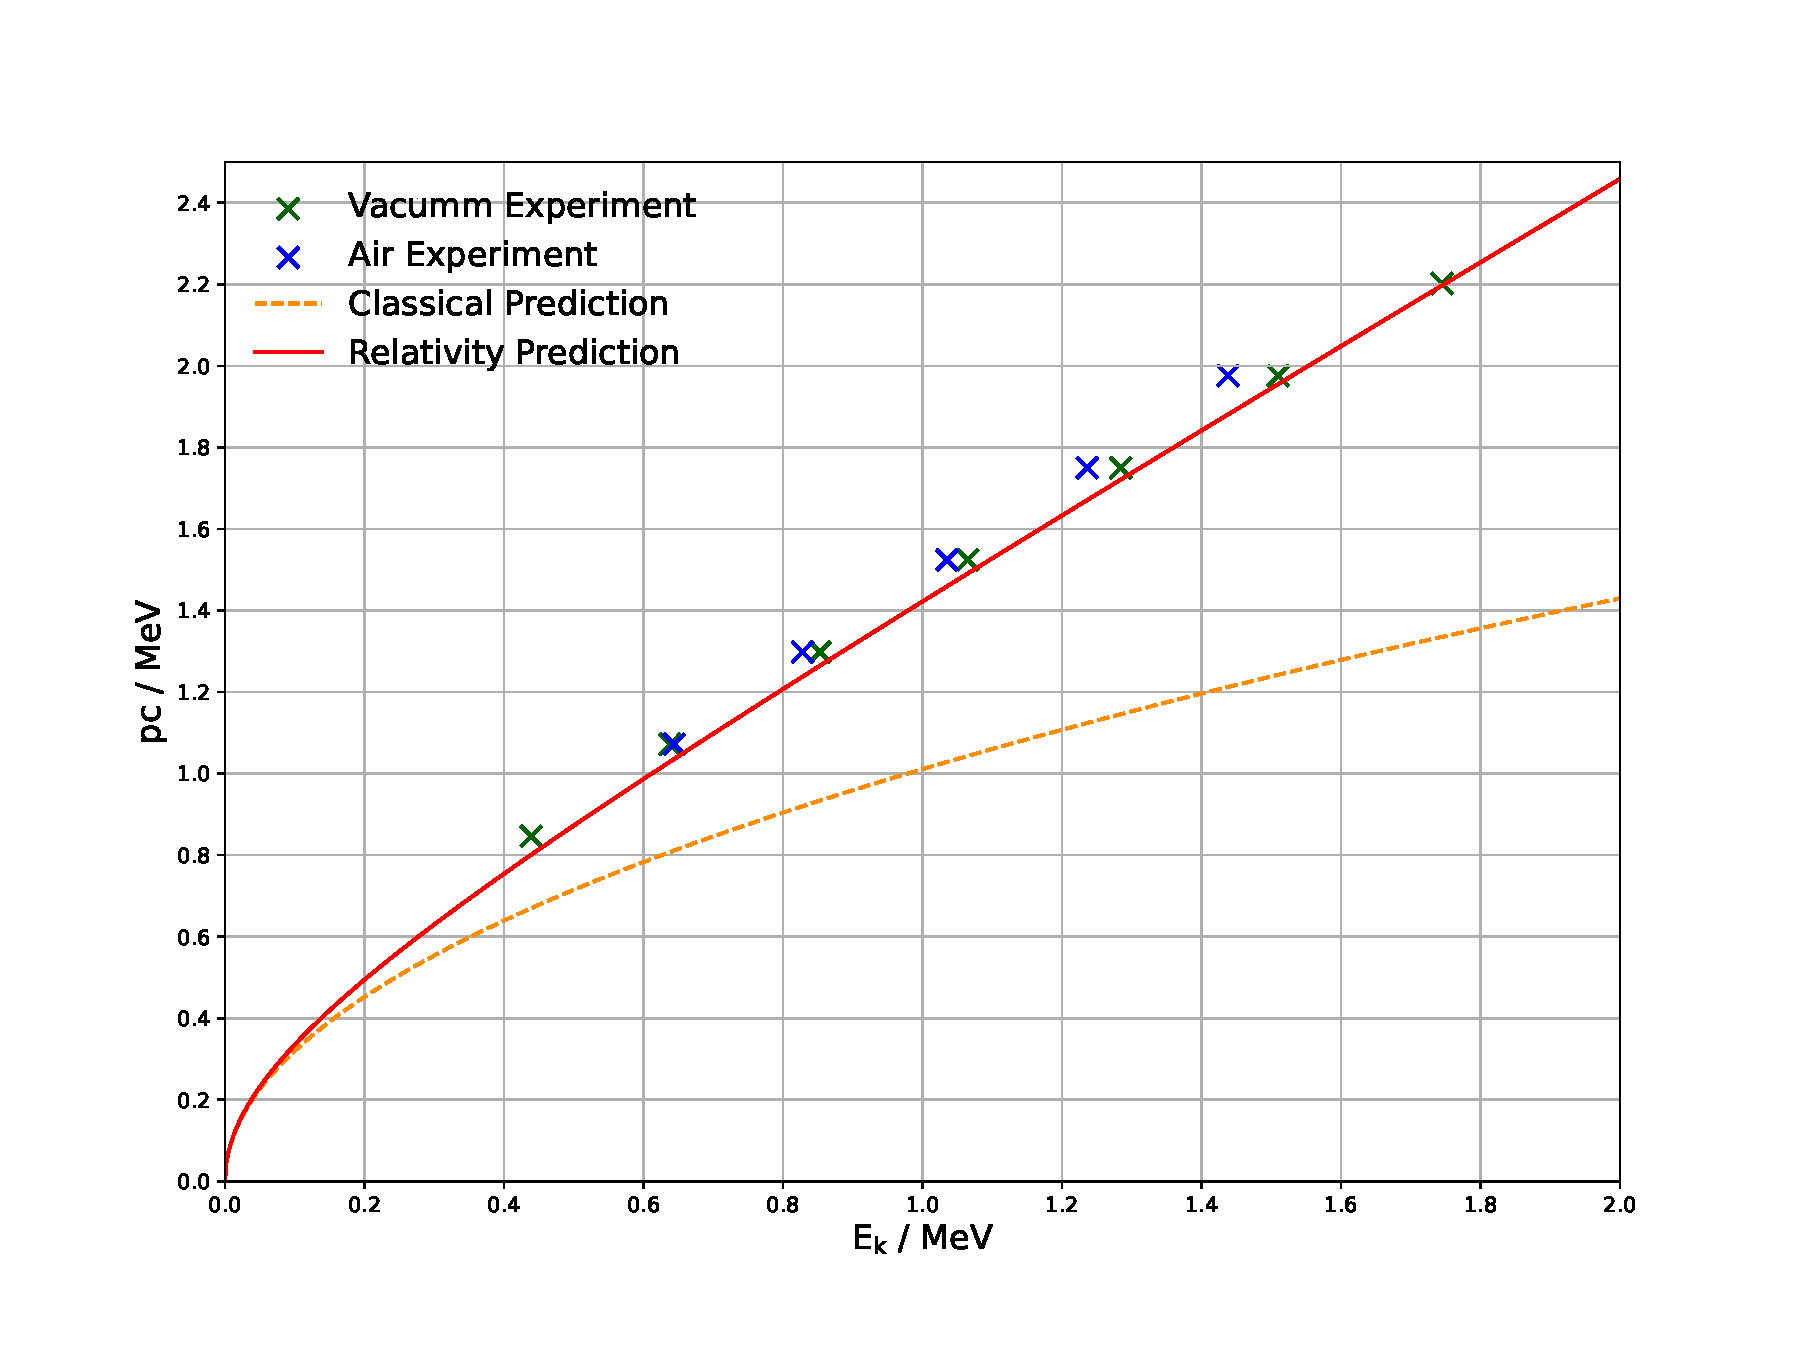
\includegraphics[height=12cm, width=16cm]{images/phyex4_fig.pdf}
 \label{fig:fig6}
\end{figure}
实验证明显然验证了相对论理论的正确性

%add more subsections for other block

%%%%%%%%%%%%%%%%%%%%%%%%%%%%%%%%%%%%%%%% Conclusion %%%%%%%%%%%%%%%%%%%%%%%%%%%%%%%%%%%%%%%%
\newpage
\section{结论}\label{conclusions}
实验证实了高能$\beta$粒子的动量--动能的关系(色散关系)满足狭义相对论的理论预测,即在误差容许的范围内,有:
\begin{equation}
	E_k = \sqrt{p^2 c^2 + m^2 c^4} - m^2 c^4
\end{equation}
	
从而初步验证了狭义相对论对高速运动物体的适用性.同时,实验结果与经典理论的严重偏离确认了经典力学对高速运动不适用.

同时可以发现,空气中测出来的峰位置和真空有偏差,导致动能跟理论预言和真空状态比起来都偏小,真空状态结果和理论预言非常相近

%%%%%%%%%%%%%%%%%%%%%%%%%%%%%%%%%%%%%%%% Questions %%%%%%%%%%%%%%%%%%%%%%%%%%%%%%%%%%%%%%%%
\begin{comment}
\section{实验报告思考题}\label{questions}
\subsection{在$a=23.0mm$、$b=10.0mm$的矩形波导管中能不能传播$\lambda=2cm$、$3cm$和$5cm$的微波?各能传播哪些波型?}\label{sub:question1}
答:根据
\begin{equation}
    \lambda_c=\frac{2}{\sqrt{(m/a)^2+(n/b)^2}}
\end{equation}
我们可以算出可传播的最大波长为$\lambda_{max}=18.3mm$,显然不能传播$\lambda=2cm$、$3cm$和$5cm$的微波,可传输波长在$\lambda_{max}=18.3mm$以下,满足$\lambda_c=\frac{2}{\sqrt{(m/a)^2+(n/b)^2}}$的波长的波型\\

\end{comment}

%%%%%%%%%%%%%%%%%%%%%%%%%%%%%%%%%%%%%%%% Acknowledgements %%%%%%%%%%%%%%%%%%%%%%%%%%%%%%%%%%%%%%%%

\section{致谢}\label{acknowledgments}
感谢王老师在实验中的的悉心指导.

\begin{comment}
%%%%%%%%%%%%%%%%%%%%%%%%%%%%%%%%%%%%%%%% Appendix %%%%%%%%%%%%%%%%%%%%%%%%%%%%%%%%%%%%%%%%
\appendix
\section{代码}\label{sub:app.code}
请在附录\ref{sub:app.code}中添加代码。请使用如下Scala的语法高亮描述方法。
\begin{scala}
class TopIO extends Bundle() {
	val boot = Input(Bool()) 
// imem and dmem interface for Tests
	val test_im_wr		= Input(Bool())
	val test_im_rd 		= Input(Bool())
	val test_im_addr 	= Input(UInt(32.W))
	val test_im_in 		= Input(UInt(32.W))
	val test_im_out 	= Output(UInt(32.W))

	val test_dm_wr		= Input(Bool())
	val test_dm_rd 		= Input(Bool())
	val test_dm_addr 	= Input(UInt(32.W))
	val test_dm_in 		= Input(UInt(32.W))
	val test_dm_out 	= Output(UInt(32.W))

	val valid			= Output(Bool())
}
class Top extends Module() {
	val io 		= IO(new TopIO())//in chisel3, io must be wrapped in IO(...) 
	//...
	when (io.boot & io.test_im_wr){
		imm(io.test_im_addr) := io.test_im_in
		} .elsewhen (io.boot & io.test_dm_wr){
		// please finish it
		} //...
}
\end{scala}
\newpage

%%%%%%%%%%%%%%%%%%%%%%%%%%%%%%%%%%%%%%%% REFERENCE %%%%%%%%%%%%%%%%%%%%%%%%%%%%%%%%%%%%%%%%
\begin{thebibliography}{9}

\bibitem{Erdos01} P. Erd\H os, \emph{A selection of problems and
results in combinatorics}, Recent trends in combinatorics (Matrahaza,
1995), Cambridge Univ. Press, Cambridge, 2001, pp. 1--6.

\end{thebibliography}
\end{comment}
\end{document}

